\chapter{Stochastic Simulation of Chemical Reactions}

Recall that a Ordinary Differential Equations is continuous and deterministic, while in contrast chemical reactions can manifest themself randomly. This will led us to the definition of stochastic simulation algorithm for chemical reactions. 

\section{Introducing randomness in chemical reactions}
Chemical reactions are not deterministic. Given for example to single molecules in a chemical solution, is difficult to predict in advance when they react. Doing it would require to know the angle and speed of the molecules, to take into account the molecules that compose the solution they are in and so on. Thus we abstract the time of the occurrence of the reaction using a \textbf{continuous probability distribution}.\par
So taking into account these information, using ODEs to represent chemical reaction seems wrong now. This is true, but if we that into account a chemical solution with an high concentrations of reactants, \textbf{the law of large numbers allow us to ignore the random aspect of our chemical reaction}. So the rule is:

\begin{itemize}
    \item \textbf{If there are a lot of molecules:} random aspects can be ignored, permitting us to use ODEs to represent the reaction.
    \item \textbf{If there are a small number of molecules:} random aspects become crucial, requiring necessary the use of \textbf{descrete variables}.
\end{itemize}

\section{Gillespie's Stochastic Simulation Algorithm (SSA)}
The Gillespie's Stochastic Simulation Algorithm is an exact procedure for simulating the time evolution of a chemical reacting system by taking proper account of the randomness inherent if such a system. \par
Consider a set of reactions $\mathcal{R} = \{R_{1}, ... , R_{n}\}$, then the SSA:

\begin{itemize}
    \item Assumes a stochastic reaction constant $c_{\mu}$ for each chemical reaction $R_{\mu} \in \mathcal{R}$.
    \item Given an infinitesimal time interval $dt$, then $c_{\mu} dt$ is the probability that a particular combination of reactants of $R_{\mu}$ react during the interval.
\end{itemize}

\subsection{Explaining $c_{\mu}$}
The constant $c_{\mu}$ is used to compute the \textbf{propensity} (also called stochastic rate) of $R_{\mu}$ to occur in the whole chemical solution $a_{\mu}$ as follows:
\begin{center}
    $a_{\mu} = h_{\mu} c_{\mu}$
\end{center}

where $h_{\mu}$ is the number of distinct molecular reactant combinations.\par

Defined $R_{\mu}$ as:
\begin{center}
    $\ell_{1} S_{1} + ... + \ell_{p} S_{p} \xrightarrow{c} \ell^{'}_{1} P_{1} + ... + l^{'}_{\gamma} P_{\gamma}$
\end{center}

The number of distinct reactant combinations of $R_{\mu}$ in a solution with $X_{i}$ molecules of $S_{i}$ with $1 \leq i \leq \rho$ is:
\begin{equation*}
    h_{\mu} = \prod^{\rho}_{i = 1} \binom{X_{i}}{\ell_{i}} 
\end{equation*}

\textbf{Note:} you can interpret the propensity as the rate of stochastic equations:\textbf{the higher is the propensity, the more often the reaction will take place}.

\subsection{Using propensity as a stochastic rate}
Propensity $a_{\mu}$ is used in Gillespie's as a stochastic rate. It is a parameter of a probability distribution used to describe the time of every reaction s.t on average I obtain a frequency which is the same as I got in the differential equation. To do so I will use the propensity in an exponential probability distribution to compute the time between subsequent occurrences of reaction $R_{\mu}$. The obtained probability distribution will tell me when the next occurrence of the reaction we have model will take place.

\subsection{What is an exponential distribution}
An exponential distribution is a continuous probability distribution that takes place in $[0, \infty]$ describing the \textbf{timing between events} in a Poisson process, namely a process in which events occur continuously and independently at a constant average rate. The constant average rate is a parameter.\par

The exponential distribution is described by a negative probability density function f and by a cumulative distribution function. Both are using the parameter $\lambda$ as follows:

The probability density function $f(x)$ will tell you how likely the event will take place over time. Obviously is our case we will set $\lambda$ = $a_\mu$ (the propensity). Below the formula:
\[
f(x) =
\begin{cases}
        \lambda e^{- \lambda x} \ \ \ x \geq 0  \\
        0 \ \ \ \ \ \ \ \ \ x < 0\\
\end{cases}
\]

The cumulative distribution function that tell you the probability that the event will happen from 0 to x.
\[
F(x) =
\begin{cases}
        1 - e^{- \lambda x} \ \ x \geq 0  \\
        0 \ \ \ \ \ \ \ \ \ \ x < 0\\
\end{cases}
\]

\textbf{Note:} the mean of an exponentially distributed variable with parameter $\lambda$ is $\frac{1}{\lambda}$.

\begin{figure}[h]
    \centering
    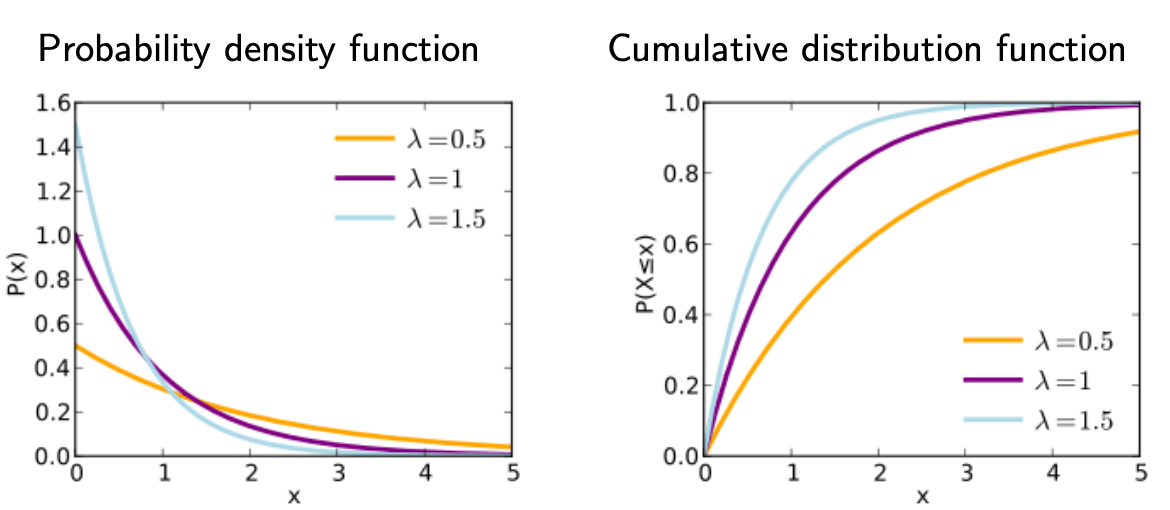
\includegraphics[width=0.8\textwidth]{Images/06 - Stochastic Simulation of Chemical Reactions/Graphs_Density_Cumulative.png}
    \caption{example of a graph for a Density Function and a Cumulative Function} 
\end{figure}

For every reaction in the set of reaction I am considering I have a propensity that is associated to a probability distribution. We can interpret reaction as parallel processes that happen recursively and the frequency of the occurrence are computed by exponential distribution

\subsubsection{Properties of exponential distribution}
There are two important properties of the exponential distribution:
\begin{itemize}
    \item \textbf{The exponential distribution is memoryless:}
        \begin{equation*}
            P(X > t + s | X > s) = P (X > t)
        \end{equation*}
        This allows a simulation algorithm in which the exponential distribution is used to forget about the history of the simulation.

    \item Let $X_{1}, ..., X_{n}$ be some independent exponentially distributed random variables with parameters $\lambda_{1}, ..., \lambda_{n}$, then the equation:
        \begin{equation*}
            X = min(X_{1}, ..., X_{n}
        \end{equation*}
        is also exponentially distributed.
        We set $\lambda = \lambda_{1} + ... + \lambda_{n}$. This allows a simulation algorithm to use a unique exponential distribution for the whole set of reactions to be simulated.    
\end{itemize}

\subsection{Introducing the algorithm}
Given:
\begin{itemize}
    \item A set of molecular species $\{S_{1}, ..., S_{n}\}$.
    \item an initial numbers of molecules of each species $\{X_{1}, .., X_{n}\}$ with $X_{i} in \mathbb{N}$.
    \item a set of chemical reactions $\{R_{1}, ..., R_{M}\}$.
\end{itemize}
Gillespie's algorithm computes a possible evolution of the system.\par
The \textbf{state} of the simulation:

\begin{itemize}
    \item is a vector representing the multiset of molecules in a chemical solution (at the start it is initialized as $[X_{1}, ..., X_{n}]$).
    \item a real variable $t$ representing the simulation time (at the start it is initialized as $t = 0$).
\end{itemize}

Then the algorithm iterates the following steps until it reaches a final value indicated as $t_{stop}$:
\begin{itemize}
    \item  The time $t + \tau$ at which the next reaction will take place. The time is randomly chosen with $\tau$ exponentially distributed with parameter $a_{0} = \sum^{m}_{v=1} a_{v}$
    \item The reaction $R_\mu$ that has to occur at time $t + \tau$ is randomly chosen with probability $\frac{a_{\mu}}{\sum^{M}_{v=1} a_{v}}$
\end{itemize}

At each step t is incremented by $\tau$ and the multiset representing the chemical solution is updated by subtracting reactants and adding products.

\subsection{Implementation details}

\subsubsection{Generation of $\tau$}
Recall that $\tau$ is randomly chosen at each step. A random number with any probability distribution can be computed froma  random number with uniform distribution by applying the \textbf{inversion sampling method}. The idea is to use the inverse of the cumulative distribution function.

Given a cumulative distribution function $F$ of a probability distribution $dist$ and a uniformly  distributed random variable $U$, the variable $X = F^{-1}(U)$ is a random variable with distribution $dist$.\par

In the case of the exponential distribution, the cumulative distribution function for $x \geq 0$ is $F(x) = 1 - e^{- \lambda x}$. Let us now invert the function:

\begin{align*}
    &F(X) = 1 - e^{- \lambda x} \Rightarrow 1 - F(x) = e^{- \lambda x}
    \Rightarrow ln(1 - F(x)) = - \lambda x \\ &\Rightarrow - \frac{1}{\lambda} ln(1 - F(x)) = x \Rightarrow \frac{1}{\lambda} ln \frac{1}{1 - F(x)} = x
\end{align*}

So we obtain:

\begin{equation*}
    F^{-1}(Y) = \frac{1}{\lambda}ln( \frac{1}{1 - Y})
\end{equation*}

Since $Y$ is uniformly distributed, also $1 - Y$ is uniformly distributed. This allows us to simplify the definition of $F^{-1}$ as:

\begin{equation*}
    F^{-1}(Y) = \frac{1}{\lambda}ln( \frac{1}{Y})
\end{equation*}

where:

\begin{itemize}
    \item $\tau$ is exponentially distributed with parameter $a_{0}$ can be computed as $\tau = \frac{1}{a_{0} ln ( \frac{1}{Y})}$ with $Y$ obtained from a standard random number generator.
\end{itemize}

\subsubsection{Choice of reaction $R_{\mu}$}
Recall that $R_\mu$ is the reaction we randomly choose to take action at the step $\tau$. First of all $R_\mu$ will be choose with probability $\frac{a_{\mu}}{a_{0}}$.\par
We do this by following these steps:
\begin{itemize}
    \item We generate a random number $N$ uniformly distributed in $[0, a_{0}$, that is $N = n * a_{0}$ with $n \in [0,1)$ obtained by using a standard number generation.
    \item we start summing $a_{1}, a_{2}, ...$
    \item as soon as the sum becomes greater than $N$, the number of completed iterations gives you $\mu$
\end{itemize}

\begin{figure}[h]
    \centering
    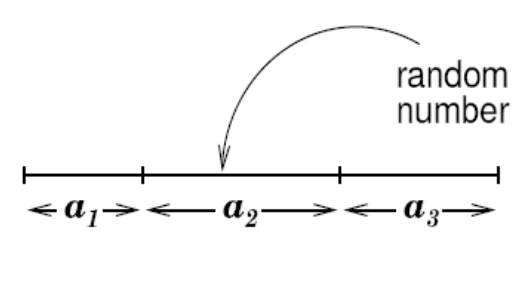
\includegraphics[width=0.5\textwidth]{Images/06 - Stochastic Simulation of Chemical Reactions/Random_Number.png}
    \caption{Choosing the random number} 
\end{figure}

\textbf{Note:} $\mu$ is the smallest integer $k$ satisfying $\sum^{k}_{i=1} a_{i} > na_{0}$ with $n$ uniformly distributed in $[0,1)$

\subsection{Computational cost of Gillespie's algorithm}
The problem of this stochastic approach is the computational cost: because I am executing reaction one by one, I have to repeat the simulation sever time to explore as many behaviour as possible, wasting a lot of time. In the case of large models this may become extremely high, like for example:

\begin{itemize}
    \item when there are large number of molecules
    \item kinetic constant are high
\end{itemize}
In respect to ODEs, this is the only disanvantage.   

\subsection{Variants}
To solve the computational drawback, several variants of Gillespie's algorithm have been introduces.

\subsubsection{Exact approaches}
\textbf{Exact approaches} are variants that improve the computation cost without introducing any approximation:

\begin{itemize}
    \item Gibson and Bruck proposed the use indexed binary tree priority queue to improve the choice of the reaction $R_\mu$ for each step.
    \item Cao et al. and McCollum et al. proposed dynamical ordering strategies for reaction propensities $a_{1}, ...$ in order to probabilistically reduce the time needed to choose $R_\mu$ at each step.
\end{itemize}

\subsubsection{Approximate approaches}
\textbf{Approximate approaches} aims to reduce the computational cost by reducing the number of steps of the overall computation:

\begin{itemize}
    \item Gillespie proposed the $\tau$-leaping method: the idea is to allow several reactions to take place in a single longer time step, under the condition that reaction rates do no change too much during that time.
    \item Gillespie et al. proposed the slow-scale Stochastic Simulation Algorithm ssSSA which separates fast reactions from slow reactions. At each step fast reactions are dealt with by assuming that they reach a dynamic equilibrium, so only their stady state is computed. Slow reaction are simulated one by one in the standard SSA.
    \item Hybrid simulation is a technique which combines ODEs with stochastic simulation: ODEs are applied to molecules occurring in big numbers, stochastic simulation to molecules occurring in small number.
\end{itemize}

\textbf{Note:} the $\tau$-leaping method is the most common.

